\section{Feedback Configurations} \label{sec:feed}

The fundamental interest of this project was to develop two novel, intuitive and useful feedback schemes to convey proprioceptive information through electrotactile stimulation and evaluate which one would aid control the most. The following section will present the two developed spatial and amplitude feedback schemes. All anatomical directions are explained with the hand being pronated as reference.      

\subsection{Spatial Configuration}

The spatial feedback scheme was created with the interest of achieving an intuitive way to convey the feedback by focusing stimulation to localized regions on the skin. An illustration of the spatial feedback scheme can be seen in \figref{fig:spatial}. The intent was to break down the number electrode pads into two groups: one upper and one lower. The upper eight pads (5-12) were used to convey information of the rotational DoF using four pads for either side.  The four pads were divided into pairs of two, where the first from the center in e.g. pronation would be activated when the cursor entered the first level in the grid system. Likewise, would the second level pair be activated when the cursor entered the second level. Hence, during a transition from neutral to level one and level one to level two, the subject should feel the stimulation moving either laterally or medially depending on the position of the cursor. Finally, this meant that when the virtual prosthesis was in a supinated state the stimulation should be felt in the anterior lateral region of the arm, while when the virtual prosthesis was is in a pronated state stimulation should be felt in the anterior medial region of the arm.   \\
The lower eight pads (1-4 and 13-16) were used to convey information about the closed hand DoF. The pads were paired in an opposite manner for each of the four levels respectively, e.i. 4 and 13, 3 and 14, 2 and 15 and 1 and 16. As the hand would move to one closed hand state out of four possible, a certain pad pair would activate. Transiting from neural to fully closed, the subject should feed the stimulation converging on the posterior side of the arm. The virtual prosthesis was able to be in states, which was a combination of the two DoFs. In these cases the feedback would be a combination of any upper and lower pair, resulting in the activation of four pads simultaneously. In the spatial feedback scheme, it was chosen to use the second amplitude threshold determined to enhance the subject's perception of the stimuli. 

\begin{figure}[H]                 
	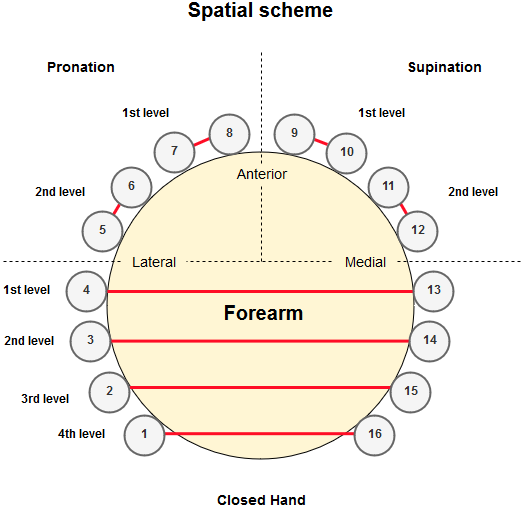
\includegraphics[width=0.55\textwidth]{figures/El_array_spatial}  
	\caption{Illustration of the developed spatial scheme, which is based on different pads being activated depending on the level of the state the cursor is located in. The level assigned to the various electrode pairs corresponded to levels of prosthesis state in \figref{fig:meth:gridmap}. The highest number of possibly activated pads was four at a time.}
	\label{fig:spatial} 
\end{figure}


\subsection{Amplitude Configuration}

Compared to the spatial configuration where the feedback was given through dynamically changing the pads activated, the amplitude configuration instead conveyed feedback in three greater regions and solely modulated the amplitude of the stimulation. The upper eight pads were again used for the rotational DoF, illustrated in \figref{fig:amplitude}. Pads 5-8 were activated at pronated states using threshold levels 2 and 3 for states 1 and 2, respectively. The same was applicable for supinated states using pads 9-12. \\
For conveying information about closed hand pads (1,2,15,16) were used. In these, threshold levels 1-4 were used for states 1-4, respectively. When in a grid position corresponding to a combined DoF prosthetic state, eight electrodes would be active in amplitude levels relative to the grid position. \\ In this scheme, attention to the recognition of stimulation localization should be less. Instead, the subject would have to focus on discriminating between the intensity of stimulation in the regions which were active.          

\begin{figure}[H]                 
	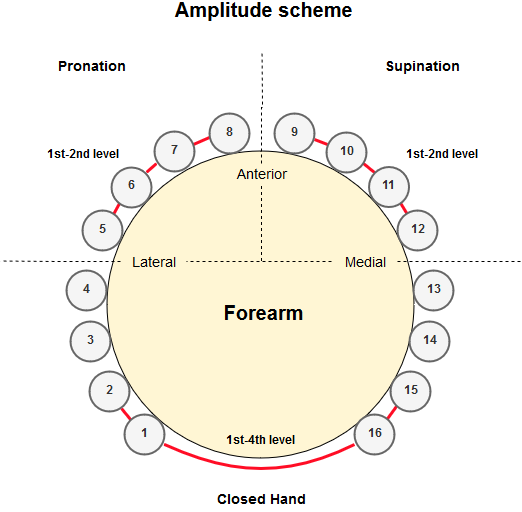
\includegraphics[width=0.55\textwidth]{figures/El_array_amplitude}  
	\caption{Illustration of the developed amplitude scheme. Here, the amplitude of the active pads would increase with the increase of the prosthetic state; the higher the level the higher the current amplitude of the given electrodes. The level of amplitude strength assigned to the various electrodes corresponded to levels of prosthesis state in \figref{fig:meth:gridmap}. The highest number of possibly activated pads was eight at a time.}
	\label{fig:amplitude} 
\end{figure}






